\section{Fiducial Region of the Measurement}\label{section:star_fiducial}
A fiducial phase space of measurement  is defined by the~following criteria. Primary charged particles are defined as charged particles with a mean lifetime $\tau >300$~ps, either directly produced in $pp$ interaction or from subsequent decays of directly produced particles with $\tau <30$~ps. In this analysis, primary charged particles had to be contained within the kinematic range of $p_\textrm{T}>0.2$~GeV/c and $|\eta|<0.7$.
The~results are corrected to the~region of the total number of primary charged particles (without identification), $2\leq n_\textrm{ch} \leq 8$.  In identified charged antiparticle to particle ratio measurement, the lower transverse momentum limit was set for the analyzed particles as follows: $0.2$~GeV/c (pions), $0.3$~GeV/c (kaons), $0.4$~GeV/c (protons and antiprotons).

The measurements were performed in a fiducial phase space of the forward scattered protons of $0.04<-t<0.16$~GeV$^{2}$/c$^2$ and $0.02 < \xi<0.2$. Figure~\ref{fig:STARtrueMCfiducial} shows that the~efficiency  to events containing at least two primary charged particles, $\epsilon_{n_\textrm{ch}\geq 2}(\log_{10}\xi)$  is larger than $50\%$ for events with $\xi>0.02$. % and for this reason the~lower $\xi$ cut was introduced. %On the other hand, the~upper $\xi$ cut was required since the~region of larger $\xi$ is dominated by \ac{DD} and \ac{ND}. 
All measured observables are presented in three $\xi$ regions: $0.02<\xi<0.05$, $0.05<\xi<0.1$ and $0.1<\xi<0.2$.

\begin{figure}[h!]
	\centering
	\includegraphics[width=0.8\textwidth, page=17]{chapters/dataSampleSTAR/img/true.pdf}
	\caption{$\epsilon_{ n_\textrm{ch} \geq 2}$ as a function of $\log_{10}\xi$ calculated from PYTHIA~8 (MBR).}
	\label{fig:STARtrueMCfiducial}
\end{figure}

\FloatBarrier